\section{Approach}

Our framework is shown in Figure~\ref{fig:flowchart}. Our goal is to learn a policy $\pi(s)$ that can dynamically determine a sequence of contextual classes to detect to help narrow down the search area of the query or make an early rejection, under certain budget constraint. We model it in a reinforcement learning framework by introducing the Markov Decision Process (MDP), which defines a single \textit{episode} of selecting actions for the input image $X$ and target query class $c_q$.

\begin{figure*}[htb]
\begin{center}
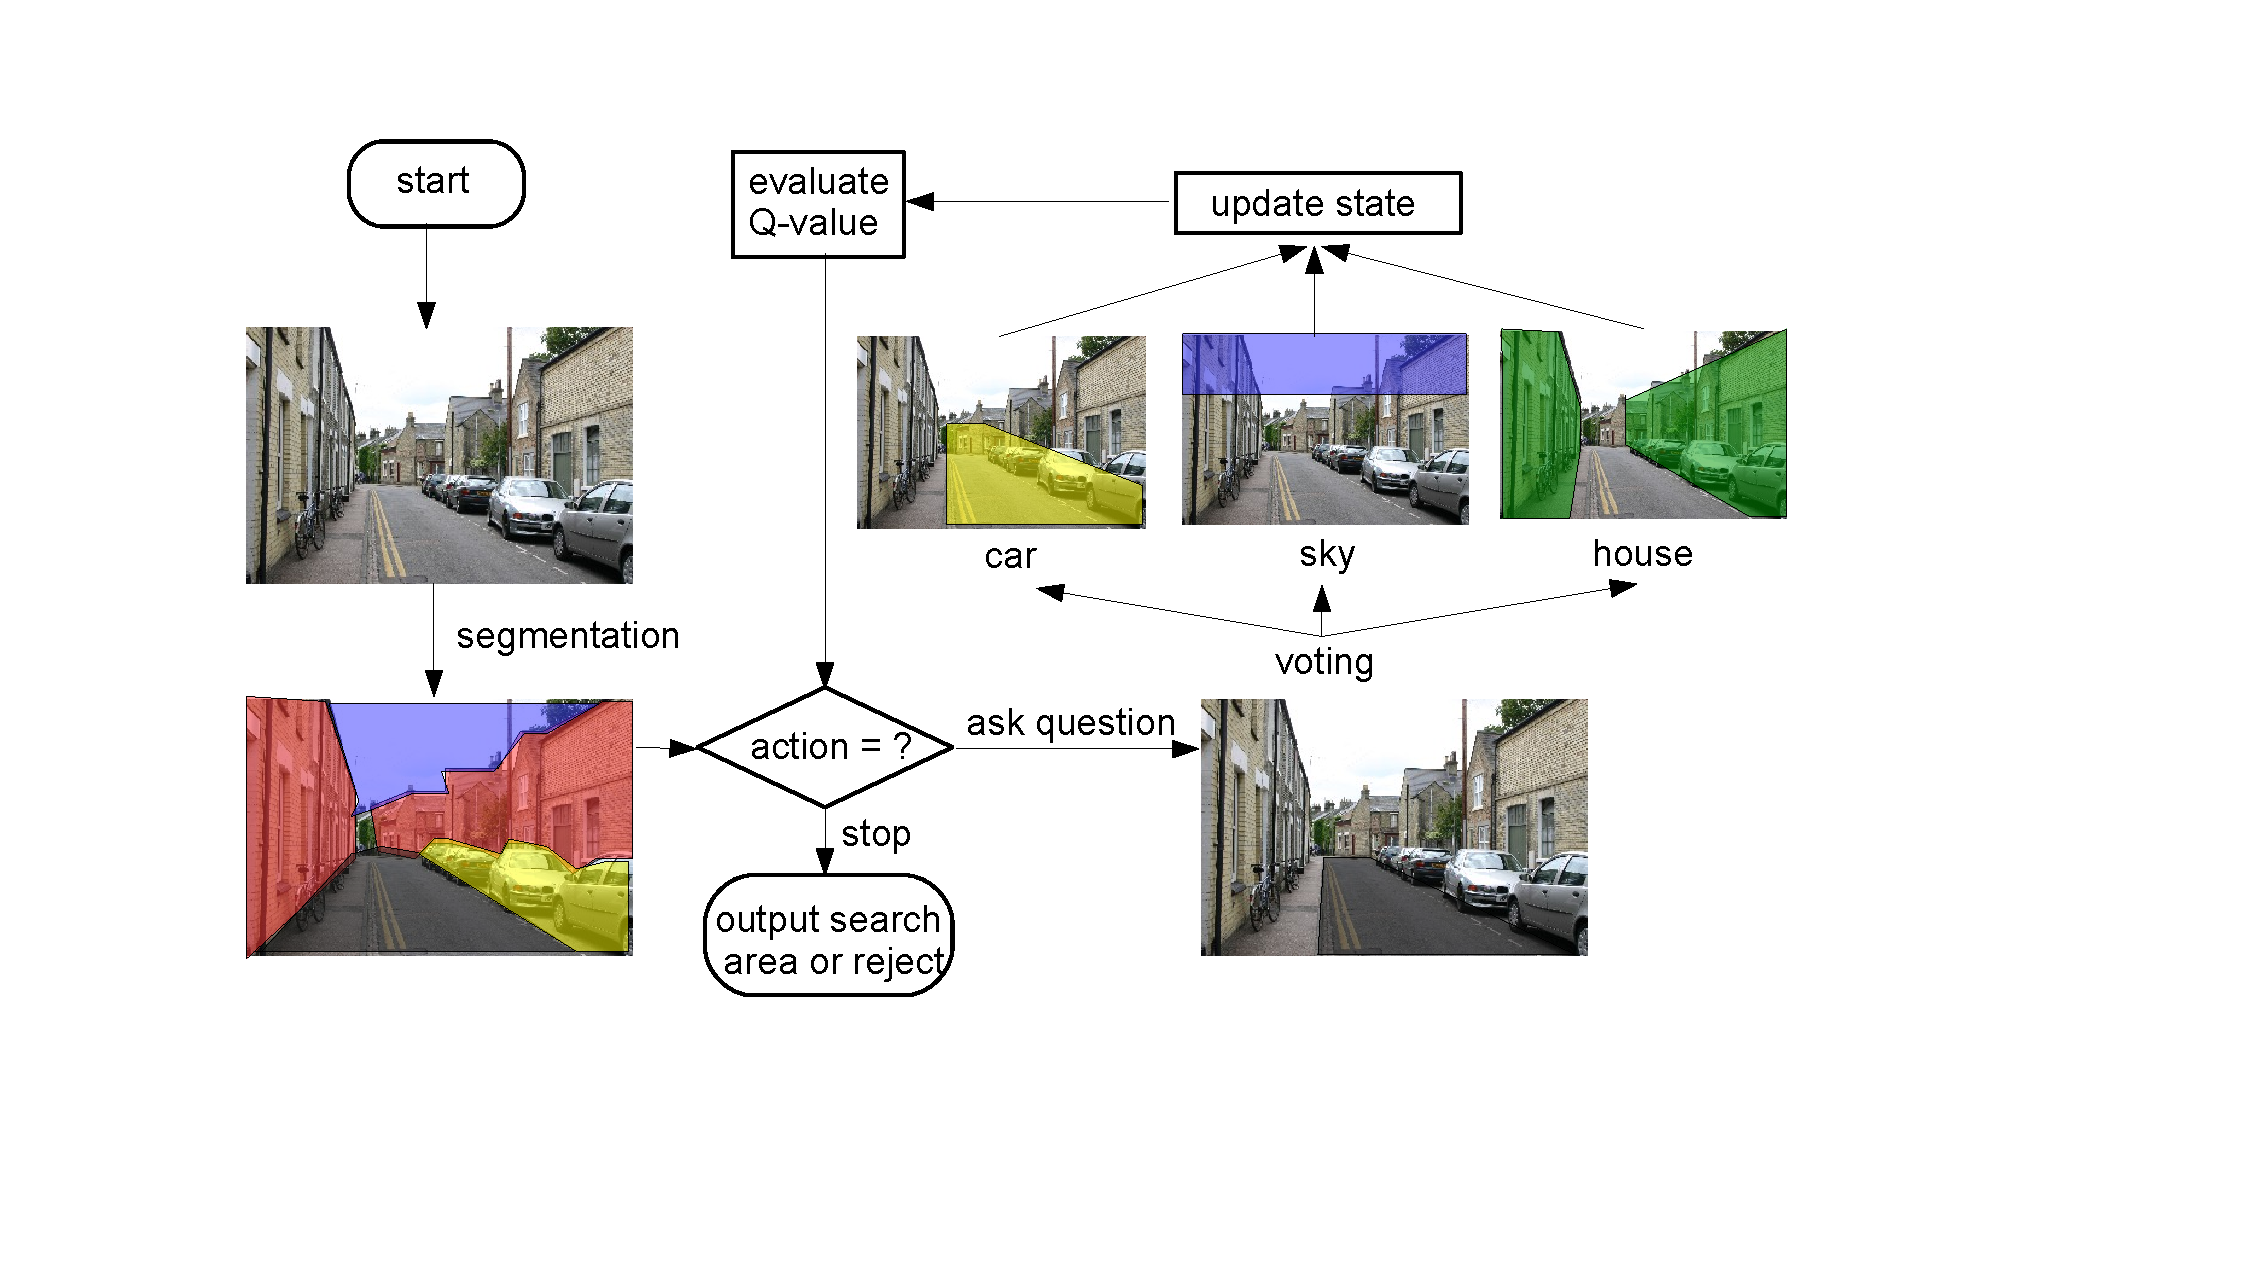
\includegraphics[width=\linewidth]{figures/flowchart_Q.pdf}
\caption{Framework of our context driven object searching. We first generate region hypotheses using object proposal algorithms, then the policy evaluates the current state and iteratively selects the action maximizing the Q-value function. Afterwards, the possible search locations are updated and the posterior probabilities of each category are evaluated for the next state.}
\end{center}

\label{fig:flowchart}
\end{figure*}

\subsection{Context Driven Object Search as Markov Decision Process (MDP)}
\label{sec:policy}

Specifically, given an image $X$ and a query object class $c_q$ in classes ${1,..,C}$, we define the MDP as follows.
\begin{mydef}
 The \textbf{detection action selection MDP} consists of the tuple $(\mathcal{S}, \mathcal{A}, T(.), R(.), \gamma)$:
\begin{itemize}
\item \textbf{State} $s(t) = (X, R^t)\in \mathcal{S}$ that includes the image $X$ and the observations $R^t= \{r_1, r_2, ....,r_t\}$ over time till $t$.
\item The set of \textbf{actions} $\mathcal{A} = \{a_1, ..., a_C, Stop, Reject\} $, where $a_i$ is to detect class $c_i$, \textit{Reject} to reject query class in the image, and \textit{Stop} to output the search area and run query detector.
\item \textbf{State transition} function $T(s'|s,a, X)$
\item The \textbf{reward} function $R(s,a,s') \rightarrow \mathbb{R}$.
\item The \textbf{discount} constant $\gamma$ defines a tradeoff between taking the action by greedily maximizing the immediate reward or the considering the long term expected reward.
\end{itemize}
\end{mydef}

%\newtheorem{def}[thm]{Definition}
% \begin{def}
% 
% \end{def}

During test time, our search policy $\pi(s): \mathcal{S} \rightarrow \mathcal{A}$ iteratively selects an action $a^t$ in the action space $\mathcal{A}$. %= \{a_1, ..., a_C, Stop, Reject\} $, . 
Then the policy obtains response $r_t$ at time step $t$ given by the detection or classification results of action $a_t$. 

Formally, since we would like to select the actions dynamically, we want to learn a value function taking action $a$ in state $s$ under the policy $\pi$, denoted $Q^\pi(s,a): S\times A \rightarrow \mathbb{R}$, where $S$ is the space of all possible states, to assign a value to a potential action $a\in A$ given the current state. We can then define policy $\pi$ to take the action that maximizes the expected value:

\begin{eqnarray}
\label{eq:pi}
\pi(s) = \arg\max_{a_i\in A\backslash R} Q(s,a_i)
\end{eqnarray}

\subsection{Reward Function}

We define the \textit{immediate reward} $R$ as the immediate gain in intersection/union of the search space after conducting action $a_i$ at time step $t$ under state $s$ as:

\begin{eqnarray}
\label{eq:imreward}
R(s^t,a_i) =  \frac{X^{t+1}_i \cap X_q}{X^{t+1}_i \cup X_q} - \frac{X^{t}_i \cap X_q}{X^{t}_i \cup X_q}
\end{eqnarray}
where $X^{t+1}_i$ is the updated search area after executing action $a_i$ in state $s_t$, determined by the context models described in Section~\ref{sec:context}. $X_q$ is the groundtruth mask of the query object instances in the image. 
  
%at each time step $t$, we select a question $q_t$ and take action $a_t$ to evaluate it. Let $R^t = \{r_1, r_2, ....,r_t\}$ be the observations of responses to the actions taken at time $1...t$, where the response $r_t = p(c_t|X)$ is the detection or classification probability of class $c_t$ corresponding to question $q_t$. 




\subsection{Learning Context Driven Search Policy}
We propose a policy to use maximum expected reward to select $a_t$. To learn such a policy, we adopt a standard Q-learning algorithm~\cite{barto1998reinforcement}, where the action-value function is estimated by using the Bellman equation iteratively:
\begin{eqnarray}
\label{eq:bellman}
Q^*(s,a) = \mathbb{E}_{s'\sim \xi} \big[ R + \gamma \max_{a'} Q^*(s',a')|s,a \big]
\end{eqnarray}
where $a'$ and $s'\in\xi$ is the possible action-state pairs at the next time steps $t+1$.

Since the space of possible states $S$ is intractable, we use a linear function of the features of the states to approximate the $Q$-values:
\begin{eqnarray}
\label{eq:qvalue}
Q^{\pi}(s,a) = \theta_\pi^T \phi(s,a) 
\end{eqnarray}

where $\phi(s,a) = \phi((X, R^t),a) = \phi(X^t,a)$ is the feature of the undetermined area $X^t$ at time $t$ after observing detector responses of $a_1,...,a_t$. 

The parameters $\theta_\pi$ are learned by \textit{policy iteration}. We collect $(s,a,r,s')$ samples by running episodes starting from a random or empty state, then we search and prune in the tree of states and collect states samples  and corresponding features. An SVM regression is trained for each class to predict the Q-values given current states.

\subsection{Context Modeling}
\label{sec:context}
Since our task is not only to detect the object but also refine the search space of the query in the image as accurately as possible, conventional modeling of context as simple co-occurrence statistics is inadequate. Instead we present a data-driven location aware approach to represent the spatial correlation between the objects and the scene. 

Here we formulate the context $p(c_t|c,X)$ as a posterior of the probabilistic vote map $p(c|c_t,X_s)$ defined on each pixel $(x_i,x_j)\in X$ over the image, and the responses of class $c_t$ after action $a_t$:
\begin{eqnarray}
p(c_t|c,X) = \sum_{s\in X^t} p(c|c_t,X_s)p(c_t|X_s)
\end{eqnarray}

Given a refined search space $X^t\in X$ of a context class $c_t$ at time $t$, we formalize $p(c|c_t,X)$ as a weighted vote from the cooccurring region pairs of class $c_t$ and $c$ in training scenes. Let $(s_{c_t}^i, s_c^i)$ be the $i$-th pair of co-occurring regions of class $c_t$ and $c$, and $b_{c_t}^i$ and $b_c^i$ be the corresponding bounding boxes. We can now define the probabilistic vote map $p(c|c_t,X)$ as:
\begin{eqnarray}
\label{eq:votemap}
p(c|c_t,X_s)_{s\in X^t} = \frac{1}{Z_c}\sum_i W(s_{c_t}^i,s;\theta^W).T(b_{c_t}^i,b_c^i)
\end{eqnarray}
where $s\in X^t$ is a region within the search space of the context class $c_t$. $Z_c$ is the normalization function. $W(.)$ is a kernel measuring similarity of region $s$ with a training region $s_i$. $T(b_{c_t}^i,b_c^i)$ models the transformation from $b_{c_t}^i$ to $b_c^i$, including translation and scaling. Figure~\ref{fig:votemap} shows a few examples of the vote maps. We can see that with the exemplar based and semantically aware voting, the resulted vote maps give more accurate search area of the query objects.


\begin{figure}[ht!]
\begin{center}
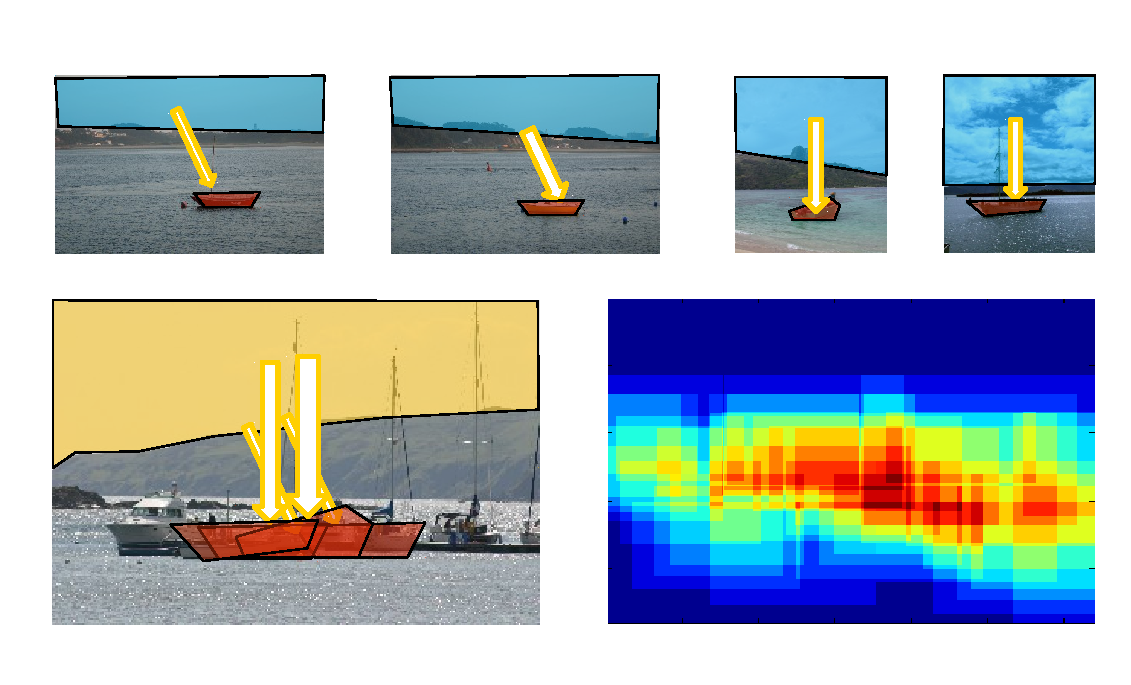
\includegraphics[width=\linewidth]{figures/vote_sky_boat.pdf}
\end{center}
\caption{Examples of our weighted vote map for the context from sky to boat. The first rows are the training sample pairs of sky and boat and the second row is the test image and the resulted weighted voting map. The widths of the arrows denote the weighted similarity $W(s_{c_t}^i,s;\theta^W)$ between the test segment of sky (highlighted in yellow) and a training instance of sky segment (in light blue)}
\label{fig:vote_sky_boat}
\end{figure}


\begin{figure}[ht!]
\begin{center}
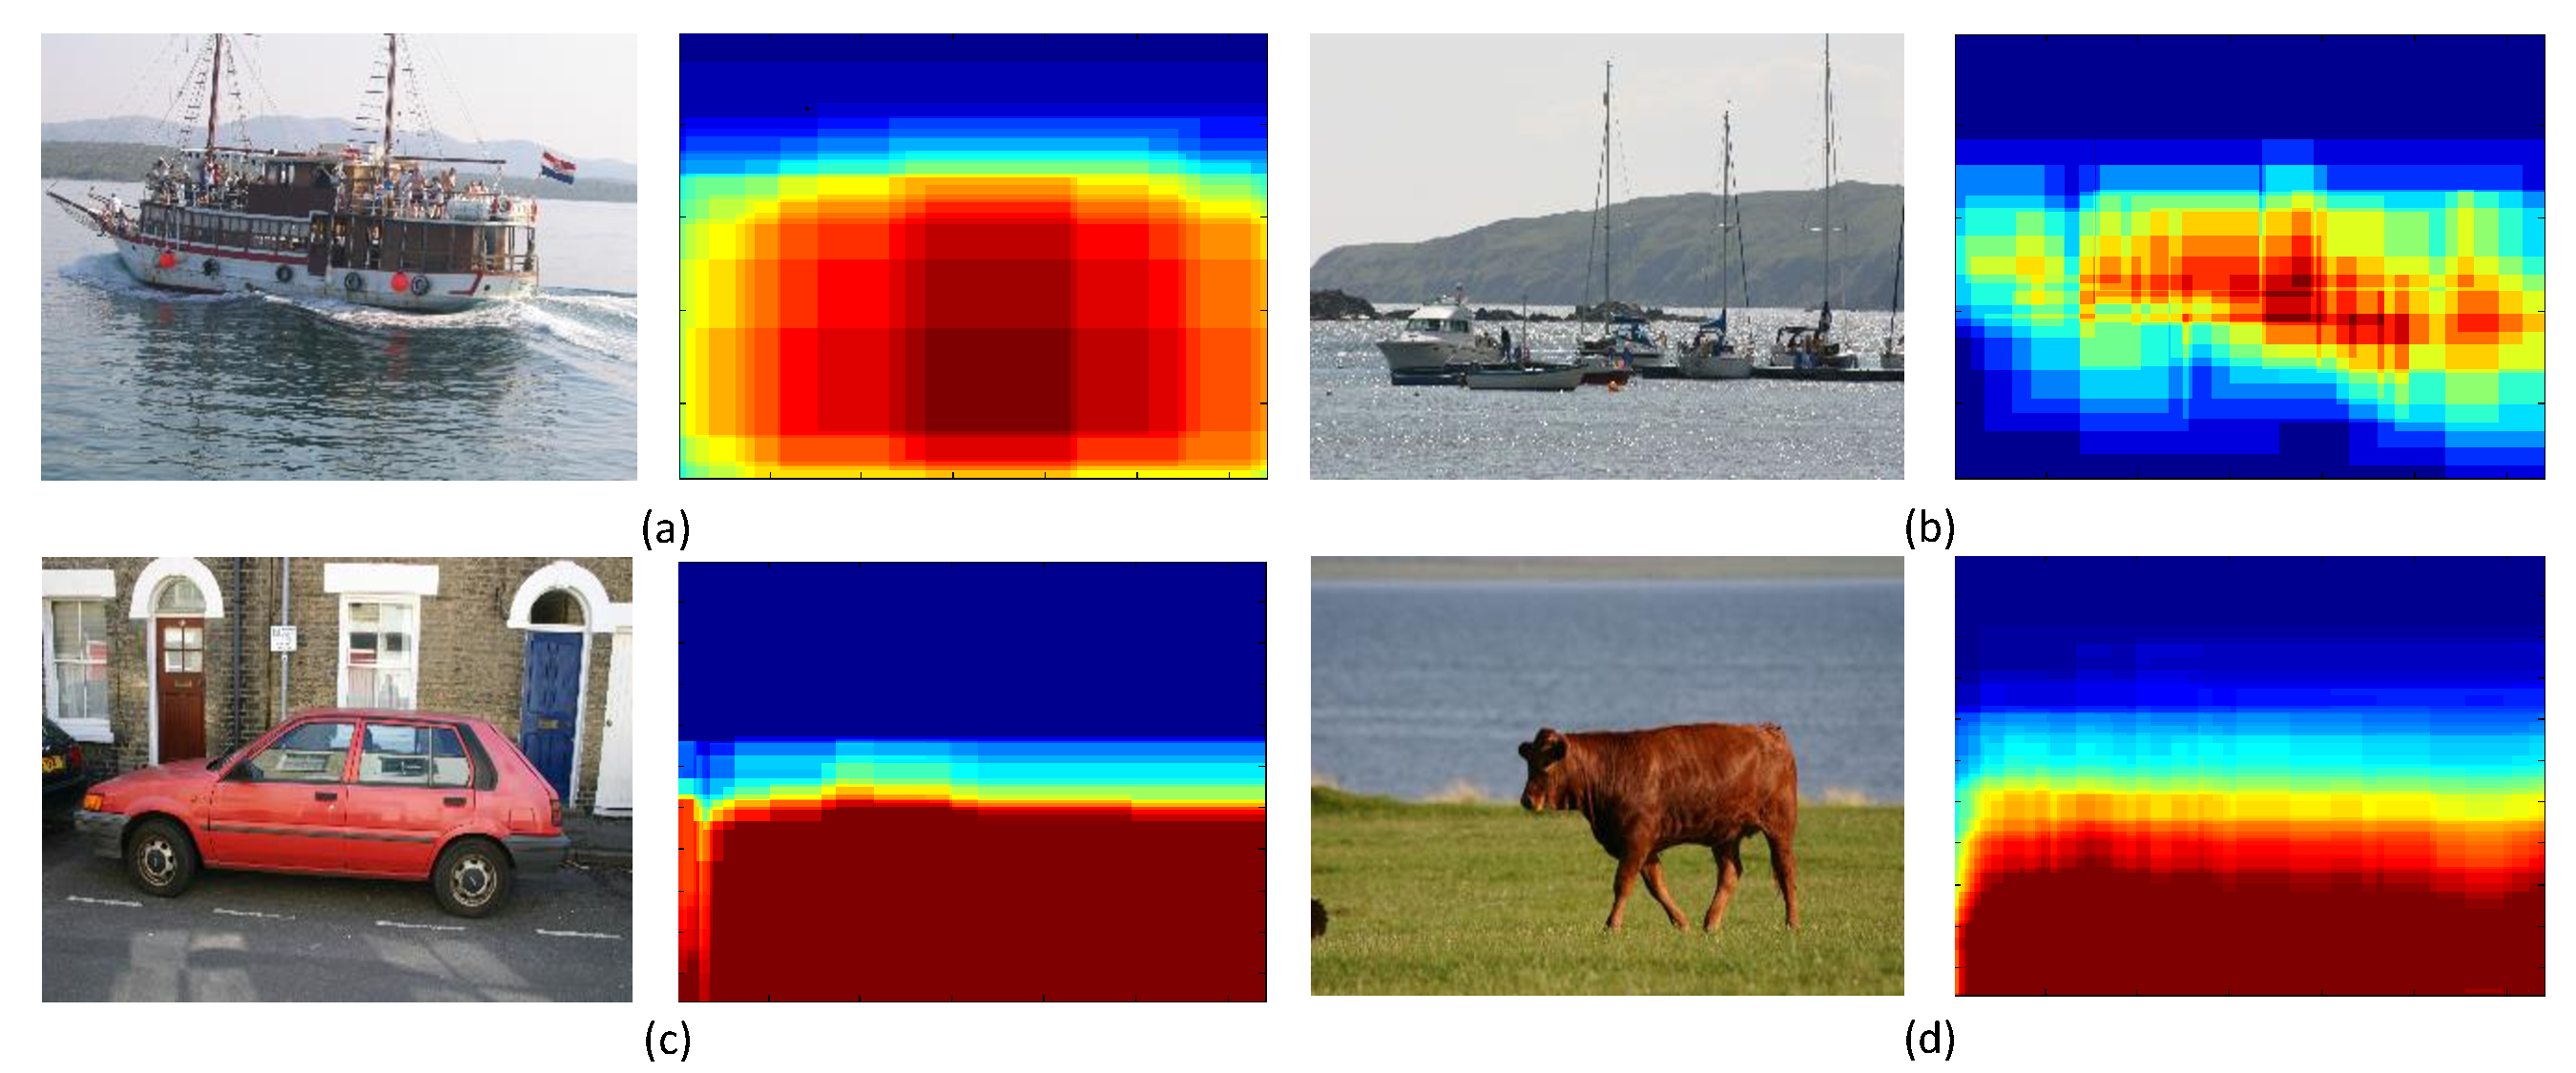
\includegraphics[width=\linewidth]{figures/votemap.pdf}
\end{center}
\caption{Examples of our context vote maps. Each pair of images corresponds to the original image and the vote-based probability map of object location from observed context. From (a) - (d) are the vote maps from water to boat, sky to boat, road to car and grass to cow, respectively. Best viewed in color.}
\label{fig:votemap}
\end{figure}



The final context probabilistic vote map is given by
\begin{eqnarray}
p(c_t|c,X) = \sum_{s\in X^t} p(c_t|X_s)\sum_i W(s_{c_t}^i,s;\theta^W).T(b_{c_t}^i,b_c^i)\nonumber\\
\end{eqnarray}
where $p(c_t|X_s)$ is the probabilities of $s$ as class $c_t$ after taking the action $a_t$ to run classification at time $t$.